\chapter{Les plaques résistives de verre de basse résistivité}
\renewcommand\chapterillustration{GLA/gla}
\ThisULCornerWallPaper{1}{\chapterillustration}
\minitoc

\lettrine[lines=4, slope=-0.5em]{C}{e} chapitre comporte une description des plaques résistives de verre de basse résisitivité ainsi que certaines de leur caractéristiques. Il comporte également les résultats obtenus lors des nombreuses campagnes de tests en faisceaux organisé au SPS, PS et Gamma Iradiation Facility (GIF++). Ces résultats ont fait l'objet d'une conférence lors de RPC2016 à ghent, de plusieurs proceeding \cite{Lagarde:2016fvf}\cite{Gouzevitch:2016pcr} ainsi que de nombreux posters.


\section{Le verre dopé de base résistivité}
Une des solution pour augmenter la capacité de détection des RPC est d'utilisé du verre de basse résistivité comme électrodes. Le nouveau verre dopé, développé par l'université de Tsinghua (Chine) présente une résitivité de l'ordre de $10^10ohms.cm$ et une très bonne uniformité de surface. Ce type de verre sera utilisé dans l'expérience \textit{Compressed Baryonic Matter} (CBM) \cite{Wang:2016bsx}. Certaines caractéristiques de ce verres sont répertorié dans le tableau \ref{tabb}
\begin{table}[H]
	\centering
	\begin{tabular}{|O|O|N}
	\hline 
	Dimenssion maximale  &32cm$\times$30cm \\ 
	\hline 
	Résistivité volumique & $10^10 ohm.cm$ \\ 
	\hline 
	Épaisseur & 0.5mm-2mm \\ 
	\hline 
	Uniformité de l'épaisseur & 0.02mm \\
	\hline
	Constante diélectrique & 7.5-9.5  \\ 
	\hline 
	Rugosité & $<10nm$ \\ 
	\hline
\end{tabular} 
\captionof{table}{Caractéristique du verre dopé.}
\label{tabb}
\end{table}
La résistivité de ces verre est 100 à 1000 fois moins importante que celle de verre standard (float glass), ce qui rend ce verre très intéressant pour la détection de particule à haut flux. La résistivité de ce matériaux se révèle également très stable même après une charge intégré de $1C/cm^2$ (cf.fig\ref{resi})
\begin{figure}[h!]
	\centering
	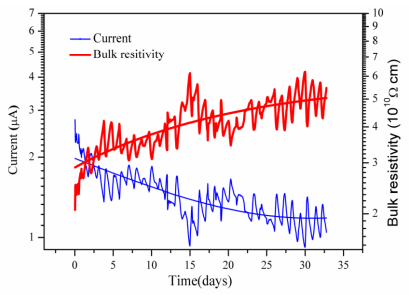
\includegraphics[width=1\textwidth]{GLA/resi.png}
	\captionof{figure}{Évolution du courant (courbe bleue) et de la résistivité volumique (courbe rouge) en fonction du temps d'une électrode de verre de basse résistivité soumise à une tension de 1000V pendant 32 jours.}
	\label{resi}
\end{figure}
La rugosité est excellente ce qui permet de n'appliquer aucun traitement de surface; contrairement au RPC en bakélite. Ces traitements se sont révélés problèmatique au cours des années.

L'inconvénient majeur de ce matériaux est sa dimension maximale qui ne peut excéder 32cm*30cm (cf.fig\ref{verre}). En effet de par le procéder de fabrication (cf.fig\ref{cooling}) de ces verres et par leur pollisage à la main, de plus grandes dimensions sont irréalisables.
\marginpar
{
	\centering
	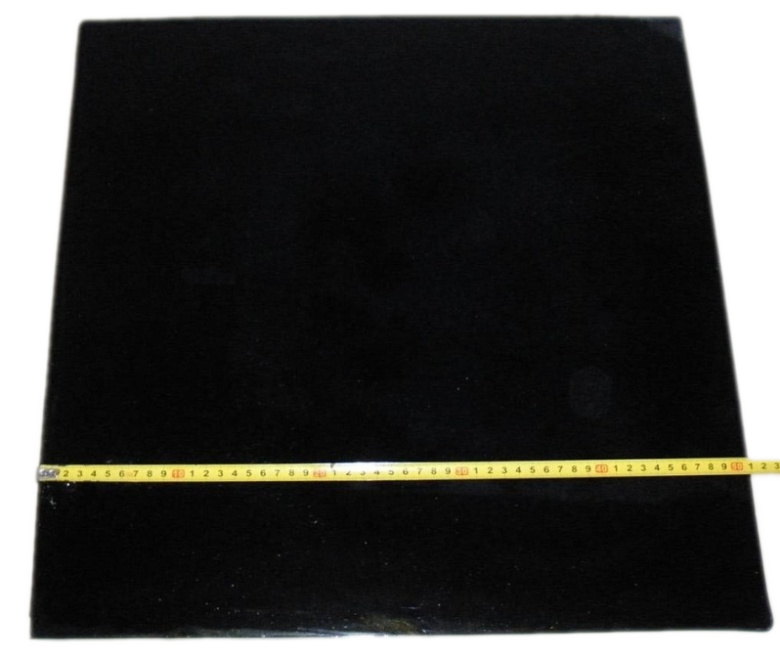
\includegraphics[width=\marginparwidth]{GLA/verre.png}
	\captionof{figure}{Photo d'une électrode de verre de basse résistivité.}
	\label{verre}
}
\marginpar
{
	\centering
	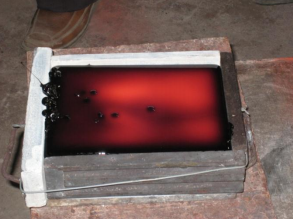
\includegraphics[width=\marginparwidth]{GLA/cooling.png}
	\captionof{figure}{Refroidissement d'un bloc de verre de basse résistivité.}
	\label{cooling}
}

Des détecteurs de cette dimension ont donc été construit afin d'étudier leur caractéristiques et de voir s'ils étaient compatibles avec les demandes de CMS.

\section{Caractérisation des Glass Resitive Plate Chamber (GRPC)}
 
L'étude des GRPC passe par la connaissance de trois caractéristique principales :
\begin{itemize}[label=$bullet$]
	\item \textbf{L'Efficacité} de détection des particules. C'est la caractéristiques principales. Elle est calculée en faisant le rapport entre le nombre de particules ayant été détectées et le nombres de particules ayant traversée le détecteur. Bien sûr, dans le cas où le signal est récolté par une électronique à seuil, la valeur de celui-ci va affecter l'efficacité de détection.
	\item \textbf{La multiplicité} représente le nombres de cellules ou bandes touchés lorsqu'une particule traverse le détecteur. En effet, plusieurs cellules de détections peuvent être déclenchées par le courant induit par les électrons créés lors de l'avalanche. Ici aussi le seuil appliqué à l'électronique influe sur la valeur de la multiplicité. La multiplicité joue un rôle très important sur la résolution spatiale du détecteur comme on le verra par la suite.
	\item \textbf{Le bruit électronique} qui est la fréquence de détection par l'électronique, d'un signal considéré comme non physique. Ceci peut être dû à une avalanche d'origine thermique ou radiative, par un courant dans le couche résistive etc. 
\end{itemize}

Un bon détecteur doit donc être proche d'une efficacité de 100\% avec une fréquence de bruit très basse. La multiplicité idéale dépend de la taille des cellules, du seuil appliqué et surtout de la résolution spatiale que l'on veut atteindre. D'autres caractèristiques du détecteurs sont imporatntes telles que la sensibilité au bruit de fond (photon et neutrons par exemple) et l'évolution des caractéristiques du détecteurs en fonction du temps, ce que l'on appelle le vieillissement du détecteurs.

Ces détecteurs ont été instrumenté avec une électronique dite semi-digitale utilisé depuis de nombreuses années aux laboratoire dans un prototype de calorimètre hadronique semi digitale (SDHCAL) (cf.fig\ref{SDHCAL}) \cite{Buridon:2016ill} pour le détecteur International Large Detector (ILD) (cf.fig\ref{ILD}); L'un des deux détecteurs de l'expérience International Linear Collider (ILC) (cf.fig\ref{ILC}).
\marginpar
{
	\centering
	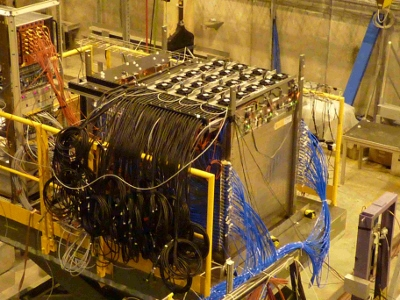
\includegraphics[width=\marginparwidth]{GLA/SDHCAL.jpg}
	\captionof{figure}{Photo du prototype SDHCAL construit à Lyon.}
	\label{SDHCAL}
}
\marginpar
{
	\centering
	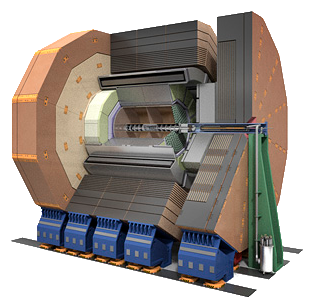
\includegraphics[width=\marginparwidth]{GLA/ILD.png}
	\captionof{figure}{Schéma de l'ILD.}
	\label{ILD}
}
\marginpar
{
	\centering
	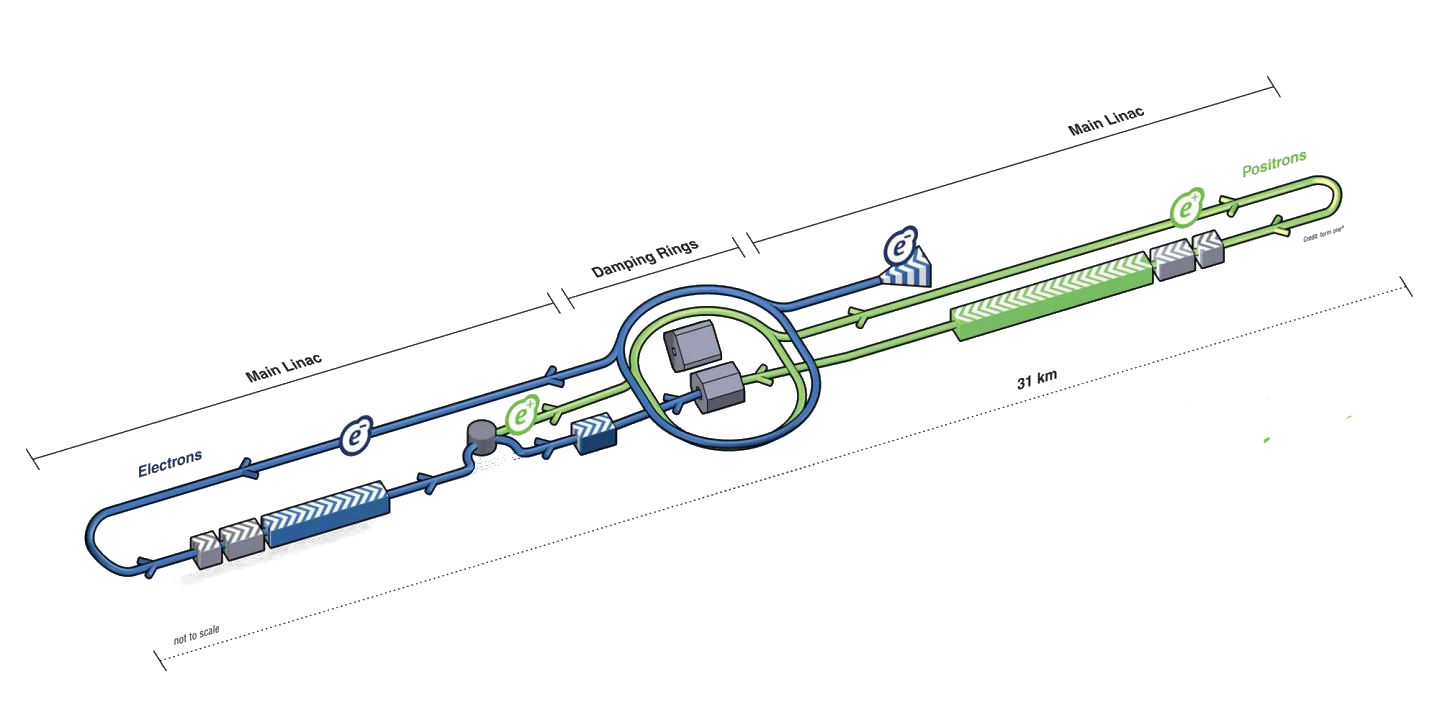
\includegraphics[width=\marginparwidth]{GLA/ILC.png}
	\captionof{figure}{Schéma de l'accélérateur ILC.}
	\label{ILC}
}